% !TeX root = ../main.tex
\begin{tikzpicture}[scale=1.2, 
	mynode/.style = {rectangle, align=center,font={\tiny}},
	myalertnode/.style = {rectangle, align=left,font={\tiny},text=mLightBrown},   -stealth
	]
	\node (data) at (-3,0) {
\includegraphics[height=40px]{images/data.png}};
	\node[above = -0.1cm of data] (datatitle) {Dataset}; 
	
	\node (trainingset) at (0,1) {
\includegraphics[height=30px]{images/data.png}};
	\node[above = -0.1cm of trainingset] (trainingtitle) {Training data};
	
	\node (testset) at (0,-1) {
\includegraphics[height=30px]{images/data.png}};
	\node[below = -0.1cm of testset] (testtitle) {Test data};
	
	\node (initmodel) at (-3,3) {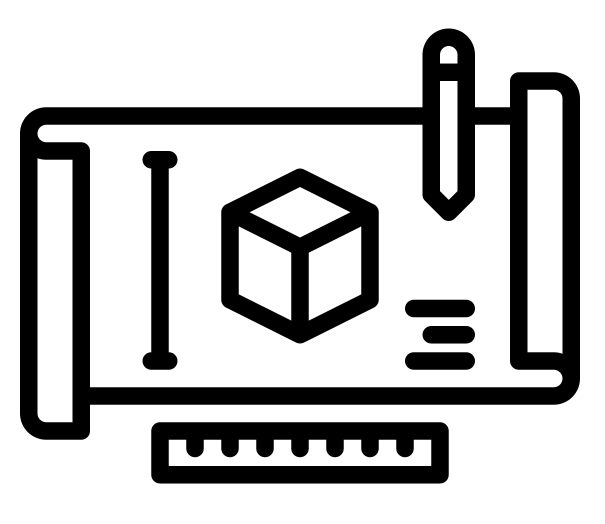
\includegraphics[height=40px]{images/noun-blueprint.png}};
	\node[above = -0.1cm of initmodel] (modeltitle) {Model architecture}; 
	
	\node (currentmodel) at (3,3) {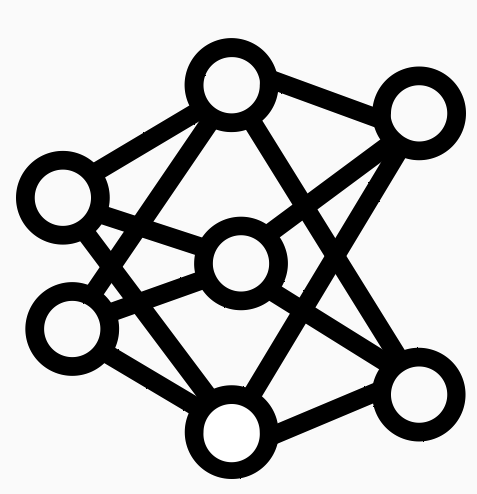
\includegraphics[height=30px]{images/model.png}};
	\node[above = -0.1cm of currentmodel] (currentmodeltitle) {Current Model}; 
	
	\node (shuffle) at (3,1) {
\includegraphics[height=30px]{images/data.png}};
	\node[above = -0.1cm of shuffle] (shuffletitle) {Shuffled data}; 
	
	\node (training) at (6,2) {
\includegraphics[height=40px]{images/noun_data_processing.png}};
	
	\node (Training loop) at (6,4) {\Large{\textbf{Training loop}}}; 
	
	\node (trainedmodel) at (9,2) {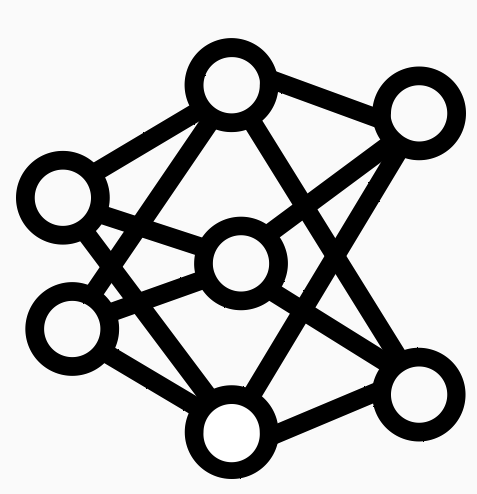
\includegraphics[height=30px]{images/model.png}};
	\node[above = -0.1cm of trainedmodel] (modeloutputtitle) {Final  Model}; 
	
	\node (evaluation) at (9,-1) {
\includegraphics[height=30px]{images/noun_evaluate.png}};
	\node[below = -0.1cm of evaluation] (evaluationtitle) {Evaluation}; 
	
	\node[right = 0.4cm of data]  (splitting) {\colorbox{blue!20}{\color{blue} \textbf{(a) Data splitting}}};
	
	\draw[rounded corners](1.5,0.2)--(7.5,0.2)--(7.5,4.3)--(1.5,4.3)--cycle;
	
	\draw[-stealth,ultra thick] (data.east) -- (trainingset.west);
	\draw[-stealth,ultra thick] (data.east) -- (testset.west);
	
	\draw[-stealth,ultra thick] (trainingset.east) -- (shuffle.west);
	\draw[-stealth,ultra thick] (initmodel.east) -- node[above] {\colorbox{blue!20}{\color{blue} \textbf{(b) Initialization }}} (currentmodel.west);
	
	\draw[-stealth,ultra thick] (training.east) -- (trainedmodel.west);
	
	\draw[-stealth,ultra thick] (testset.east) -- (evaluation.west);
	\draw[-stealth,ultra thick] (trainedmodel.south) -- (evaluation.north);
	
	
	\begin{scope}[transform canvas={yshift=.7em}]
		\path[-stealth,ultra thick, shorten <=2mm, shorten >=2mm] (currentmodel.east) edge[bend left] (training.west);
		\path[-stealth,ultra thick, shorten <=2mm, shorten >=2mm] (training.west)  edge[bend left] (currentmodel.east) ;
	\end{scope}
	
	\path[-stealth,ultra thick, shorten <=2mm, shorten >=2mm] (shuffle.east) edge[bend left] (training.west);
	\path[-stealth,ultra thick, shorten <=2mm, shorten >=2mm] (training.west)  edge[bend left] node[below right] {\colorbox{blue!20}{\color{blue} \textbf{(c) (Re)shuffling}}} (shuffle.east) ;
	
	
	\draw[-stealth,ultra thick] (testset) -- (evaluation.west);
	
\end{tikzpicture}